\documentclass{article}

% if you need to pass options to natbib, use, e.g.:
% \PassOptionsToPackage{numbers, compress}{natbib}
% before loading nips_2016
%
% to avoid loading the natbib package, add option nonatbib:
% \usepackage[nonatbib]{nips_2016}

\usepackage[final]{nips_2016}

% to compile a camera-ready version, add the [final] option, e.g.:
% \usepackage[final]{nips_2016}

\usepackage[utf8]{inputenc} % allow utf-8 input
\usepackage[T1]{fontenc}    % use 8-bit T1 fonts
\usepackage{hyperref}       % hyperlinks
\usepackage{url}            % simple URL typesetting
\usepackage{booktabs}       % professional-quality tables
\usepackage{amsfonts}       % blackboard math symbols
\usepackage{nicefrac}       % compact symbols for 1/2, etc.
\usepackage{microtype}      % microtypography
\usepackage{graphicx}
\usepackage{bm}
\usepackage{amsfonts,amssymb}
\usepackage{amsmath}
\usepackage[linesnumbered, ruled]{algorithm2e}
\usepackage{float}
 
\bibliographystyle{plain}

\title{Data Difficulty Specified Crowdsourcing}

% The \author macro works with any number of authors. There are two
% commands used to separate the names and addresses of multiple
% authors: \And and \AND.
%
% Using \And between authors leaves it to LaTeX to determine where to
% break the lines. Using \AND forces a line break at that point. So,
% if LaTeX puts 3 of 4 authors names on the first line, and the last
% on the second line, try using \AND instead of \And before the third
% author name.

\author{
  Yilun Xu, Tianyuan Zhang \\%\thanks{Course project} \\
  School of EECS\\
  Peking University\\
  \texttt{\{1600011072, 1600012888\}@pku.edu.cn} \\
  \And
  Dinghuai Zhang\\
  School of Mathematical Sciences\\
  Peking University\\
  \texttt{1600013525@pku.edu.cn}\\
  \And
  Weiyi Zhang\\
  Yuanpei College\\
  Peking University\\
  \texttt{1600017749@pku.edu.cn}
  }
\usepackage{xcolor}
\newcommand\yx[1]{\textcolor{cyan}{[Yilun Xu: #1]}}
\begin{document}
% \nipsfinalcopy is no longer used

\maketitle

\begin{abstract}
  Crowdsourcing has become a popular paradigm for collecting labels of large-scale datasets. However, the collected labels are noisy out of the inaccuracy of experts, and thus we need to aggregate labels to complete a supervised problem. Traditional methods often fail because of the complexity and non-convexity of the log-likelihood function. In this paper, we suppose the experts are people with different ability and the each data point has unique difficulty. Then we tackle the problem via EM algorithm together with our original difficulty processing method. Furthermore, we investigate our algorithms in three aspects and show the superiority of our method through ablation study with synthesized data and real data.\footnote{We choose Track A for our project.}
\end{abstract}

\section{Introduction}
In this data-driven time, the need for large-scale data has become more urgent than any time in history. Crowdsourcing comes up to solve the problem under such background, collecting labels from crowds to accomplish this mission cosmically. As the name suggests, most crowdsourcing services resort to labeling redundancy, collecting multiple labels from different workers for each item.  Though this solution seems appropriate, new problem emerges that the labeled data coming from crowds are always noisy out of non-consistency of workers' ability or the high difficulty of certain task like age estimation or medical images annotation. Under such scenario, several problems are raised:
\begin{itemize}
\item how to aggregate and infer the ground truth label from the noisy crowdsourced labels?
\item how to learn an accurate classifier based on the imperfect crowdsourced but redundant labels?
\end{itemize}
Maybe the most naive way to solve this problem is \textbf{Majority Vote}, which simply assigns the label returned by the majority of the workers and learns a classifier with the majority answer. But biased answer can be obtained with a difficult task when most experts get wrong while capable experts who give the correct answers are in the minority, causing it to be an error-prone algorithm.

More sophisticated algorithms come with more assumptions about how labels are generated from experts. A classical method proposed by \cite{dawid1979maximum} assumes that all samples have the same difficulty for each worker. With this assumption they solve a maximum likelihood problem based on the EM algorithm. Formally, they assume that each worker is associated with a $2\times 2$ confusion matrix, where the (c',c)-th entry represents the probability that a random chosen item in class c' is labeled as class c by the worker: 
\begin{displaymath}
\left( \begin{array}{cc}
\beta & 1-\beta \\
1-\alpha & \alpha  \\
\end{array} \right)
\end{displaymath}

Hereafter we denote $\alpha=\textup{Pr}[y^{\mathrm{worker}}=1|y=1]$ and $\beta=\textup{Pr}[y^{\mathrm{worker}}=0|y=0]$. 
The true labels and worker confusion matrices are jointly estimated by maximizing the likelihood of the observed labels, where the unobserved true labels are treated as latent variables.

%From the path of \cite{dawid1979maximum}, our baseline \cite{raykar2010learning} improved the algorithm with a logistic regression classifier. Besides, it extends the confusion matrix' setting to a worker-independent one. A bayesian approach is also discussed.

Obviously, there does exist data that is hard for people (worker) to deal with, and that is where the above classical algorithms fall (an example is presented in Fig \ref{fig:MNIST_confused_example1}). But taking the difficulty of each sample into consideration faces two challenges:
\begin{itemize}
    \item How to define and measure the difficulty of each sample for every experts?
    \item How to take difficulty of samples into our algorithm?
\end{itemize}

\begin{figure}[H]
    \centering
    
\includegraphics[width=3in]{image/MNIST_confused_example1.png}
    \caption{left \& middle: images that are hard to classify \quad right: image that is easy to classify} 
    \label{fig:MNIST_confused_example1}
\end{figure}

We tackle the above problem by modeling the labels generation with two assumptions:
\begin{itemize}
    \item If sample $x_i$ is more difficult than sample $x_j$, then for every experts, the probability of labeling $x_i$ wrong is bigger than making $x_j$ wrong.
    \item If expert A is better than expert B, then for every sample, the probability of expert A labeling that sample wrong is smaller than that of expert B.
\end{itemize}

Under this assumption, we design two algorithms, named \textbf{Adaptive Difficulty EM} and \textbf{Fixed Difficulty EM}. They mainly varies in the way of measuring the difficulty of each data point. We compare our algorithms with two baselines: \textbf{Majority Voting} and \textbf{Original EM} \cite{raykar2010learning} both  on synthesized and real data, we investigate these algorithms mainly in three aspects:
 \begin{itemize}
    \item How well they can estimate the ground truth
    \item The generalization of the learnt classifier
    \item How well they can estimate the expertise of each expert, i.e. sensitivity and specificity.
 \end{itemize}
 
In all above mentioned three aspects, our algorithms performs better than these two baselines.

The rest of the paper organize as follows:
Section 2 will give a brief overview of recently proposed algorithms in this area, most of them are deep free(no deep learning); Section 3 introduce the classic EM approach \cite{raykar2010learning}, then describes the details of our algorithms;  Section 4 consist of experiment setups and experiment analysis;  Section 5 gives the conclusion; Contribution is listed in the last section.



\section{Related Works}

A series of works consider crowdsourcing problem by mixing the learning process and the aggregation process together. \cite{karger2014budget} transforms the learning from crowds problem into a maximum likelihood estimation (MLE) problem, then implements an EM algorithm to jointly learn the expertise of different experts and the parameters of a logistic regression classifier. \cite{albarqouni2016aggnet} extends this method to combine with the deep learning model. \cite{khetan2017learning} also reduces the learning problem to MLE and assumes that the optimal classifier gives the ground truth labels and the experts make independent mistakes conditioning on the ground truth. Unlike our method, these MLE based algorithms are not robust to correlated mistakes. Recently, \cite{guan2018said} and \cite{rodrigues2018deep} propose methods that model multiple experts individually and explicitly in a neural network. However, their works lack theoretical guarantees and are outperformed by our method in the experiments, especially in the naive majority case. Moreover, unlike our method, their methods cannot be used to employ both the data and the crowdsourced labels to forecast the ground truth. 

Another series of methods are based on the generative model proposed by \cite{dawid1979maximum}. In particular, \cite{ghosh2011moderates} proposes a method based on Singular Value Decomposition (SVD) which addresses binary labeling problems under the one-coin model. The analysis in it assumes that the labeling matrix is full, that is, each worker labels all items. To relax this assumption, \cite{dalvi2013aggregating} proposes another SVD-based algorithm which explicitly considers the sparsity of the labeling matrix in both algorithm design and theoretical analysis. It proposed an iterative algorithm for binary labeling problems under the one-coin model and extended it to multi-class labeling tasks by converting a $k$-class problem into $k-1$ binary problems. This line of work assumes that tasks are assigned to workers according to a random regular graph, thus imposing specific constraints on the number of workers and the number of items. 

Several works focus on modeling the experts. \cite{whitehill2009whose} modeled both expert competence and image difficulty, but did not consider expert bias.
\cite{welinder2010multidimensional} models each expert as a multidimensional classifier in an abstract feature space and considers both the bias of the expert and the difficulty of the image. \cite{rodrigues2014gaussian} models the crowds by a Gaussian process. \cite{shah2016permutation} considers the generalized Dawid-Skene model \cite{dawid1979maximum} which involves the task difficulty. However, these works are still not robust to correlated mistakes.

\section{Our Approach}
\subsection{Traditional Two-coin Model}
Let $y$ be the actual but unobserved true label for the instance and $y^{j}$ \in $\lbrace 0,1 \rbrace$. Suppose each annotator (i.e. worker/expert) has sensitivity $\alpha^{j}$ and specificity $\beta^{j}$. Each annotator provides a version of this hidden true label based on two biased coins. If the true label is one, he flips a coin with bias $\alpha^j$ (sensitivity). If the true label is zero, he flips a coin with bias $\beta^j$ (specificity). 

The sensitivity is defined as the probability that an expert labels a positive sample as one.$$\alpha^{j}:=\textup{Pr}[y^{j}=1|y=1]$$
The specificity is defined as the probability that an expert labels a negative sample as zero. $$\beta^{j}:=\textup{Pr}[y^{j}=0|y=0]$$
If we model the classification problem using logistic regression, that is,
$$\textup{Pr}[y=1|\bm{x},\bm{\omega}]=\sigma(\bm{\omega}^{T}\bm{x})$$
where $\sigma$ denotes sigmoid function $\sigma ( z ) = 1 / \left( 1 + e ^ { - z } \right)$. With a pre-determined threshold value $\xi$, we can classify the data to "positive class" when $\textup{Pr}[y=1|\bm{x},\bm{\omega}]>\xi$ and classify it to the other class otherwise.

We wish to maximize the likelihood,
$$\textup{Pr}[\mathcal{D}|\bm{\theta}]=\prod^{N}_{i=1}\{\textup{Pr}[y_i^1,...,y_i^R|y_i=1,\bm{\alpha}]\textup{Pr}[y_i=1|\bm{x_i},\bm{w}]+$$
$$\textup{Pr}[y_i^1,...,y_i^R|y_i=0,\bm{\beta}]\textup{Pr}[y_i=0|\bm{x_i},\bm{w}]\}$$
where $\bm{\theta} = \{\bm{\alpha,\beta,\omega}\}$ and $\mathcal{D}=\left\{ \boldsymbol { x } _ { i } , y _ { i } ^ { 1 } , \ldots , y _ { i } ^ { R } \right\} _ { i = 1 } ^ { N }$. Besides, $$\operatorname { Pr } \left[ y _ { i } ^ { 1 } , \ldots , y _ { i } ^ { R } | y _ { i } = 1 , \boldsymbol { \alpha } \right] = \prod _ { j = 1 } ^ { R } \operatorname { Pr } \left[ y _ { i } ^ { j } | y _ { i } = 1 , \mathbf { \alpha } ^ { j } \right] = \prod _ { j = 1 } ^ { R } \left[ \alpha ^ { j } \right] ^ { y _ { i } ^ { j } } \left[ 1 - \alpha ^ { j } \right] ^ { 1 - y _ { i } ^ { j } }$$
Similarly,
$$
\operatorname { Pr } \left[ y _ { i } ^ { 1 } , \ldots , y _ { i } ^ { R } | y _ { i } = 0 , \beta \right] = \prod _ { j = 1 } ^ { R } \left[ \beta ^ { j } \right] ^ { 1 - y _ { i } ^ { j } } \left[ 1 - \beta ^ { j } \right] ^ { j _ { i } ^ { j } }
$$
For simplicity, we define
    \begin{align*}
        &p_i:=\sigma(\bm{\omega^T}\bm{x_i})\\
        &a_i:=\prod^R_{j=1}[\alpha^j]^{y_i^j}[1-\alpha^j]^{1-y_i^j}]\\
        &b_i:=\prod^R_{j=1}[\beta^j]^{1-y_i^j}[1-\beta^j]^{y_i^j}
    \end{align*}
The problem could be solved by EM algorithm, first we write out joint distribution between data and hidden variables:
$$
\ln \operatorname { Pr } [ \mathcal { D } , \boldsymbol { y } | \theta ] = \sum _ { i = 1 } ^ { N } y _ { i } \ln p _ { i } a _ { i } + \left( 1 - y _ { i } \right) \ln \left( 1 - p _ { i } \right) b _ { i }
$$
with $y = \left[ y _ { 1 } , \ldots , y _ { N } \right]$, thus
$$
\mathbb { E } \{ \ln \operatorname { Pr } [ \mathcal { D } , \boldsymbol { y } | \theta ] \} = \sum _ { i = 1 } ^ { N } \mu _ { i } \ln p _ { i } a _ { i } + \left( 1 - \mu _ { i } \right) \ln \left( 1 - p _ { i } \right) b _ { i }
$$
then:
\begin{itemize}
    \item \textup{E-step}. Given $\{\bm{\alpha,\beta,\omega}\}$ we compute the posterior probability
    $$\mu_i 
\propto \operatorname { Pr } \left[ y _ { i } ^ { 1 } , \ldots , y _ { i } ^ { R } | y _ { i } = 1 , \theta \right] \cdot \operatorname { Pr } \left[ y _ { i } = 1 | x _ { i } , \theta \right]
\\ = \frac{a_i p_i}{a_i p_i+b_i(1-p_i)}$$
    
    \item \textup{M-step}. By maximizing with regards to all parameters, we have closed form solution for $\bm{\alpha}$,$\bm{\beta}$.
    $$\alpha_j=\frac{\sum^N_{i=1}\mu_i y_i^j}{\sum^N_{i=1}\mu_i}, \quad \beta_j=\frac{\sum^N_{i=1}(1-\mu_i)(1-y_i^j)}{\sum^N_{i=1}(1-\mu_i)}$$
    For $\bm{\omega}$, we use the Newton-Raphson update given by $\bm{\omega}^{t+1}=\bm{\omega}^t-\eta\bm{H}^{-1}\bm{g}$,where
    \begin{align*}
        \bm{g(\omega)}&=\sum^N_{i=1}[\mu_i-\sigma(\bm{\omega^T\bm{x_i}})]\bm{x_i}\\
        \bm{H(\omega)}&=-\sum^N_{i=1}[\sigma(\bm{\omega^T x_i})][1-\sigma(\bm{\omega}^T\bm{x_i})]\bm{x_ix_i^T}
    \end{align*}
    
\end{itemize}
    

\subsection{Our Modification: Specified Data Difficulty}
In the model above, we assume that every instance is the same for a certain expert, which is obviously unrealistic. We assume $\alpha$ is correlated with factors in two dimensions, the ability of an expert and the difficulty of a classification task. In addition, we assume the form of $\alpha_{i}^{j}$ and 
$\beta_{i}^{j}$ as

\begin{align}
\alpha_{i}^{j}=\sigma\lbrace\lambda_{j}^{1}(p_{i}-1/2)^{2}\rbrace\\
\beta_{i}^{j}=\sigma\lbrace\lambda_{j}^{2}(p_{i}-1/2)^{2}\rbrace
\end{align}

where $\lambda_j^1$ and $\lambda_j^2$ are positive real numbers and $p_i=\textup{Pr}[y_i=1|x_i, \bm{\omega}]$, which is given by classifier. $\sigma(\cdot)$ denotes the sigmoid function

To make the structural assumption clear, we claim that:
\begin{itemize}
    \item In terms of the instance, if $p_i$ is close to 1/2, then the instance is close to decision boundary and thus the instance might well be hard to classify.
    \item In terms of the expert, he might have different abilities dealing with positive instances and negative ones, which implies difference between  $\lambda_j^1$ and $\lambda_j^2$. For larger $\lambda^{1}$ and $\lambda^{2}$, the expert has higher possibility to do the right classification.
\end{itemize}

In the meanwhile, we train two types of classifiers, one is logistic regression as the original paper, the other is a neural network, which is believed to perform better in complex classification task.

\subsection{Modified Learning Problem}
Given the training data $\mathcal{D}$ consisting of $N$ instances with annotations from $R$ annotators, the task is to estimate the classifier parameter $\bm{\omega}$, which can be used for future prediction, the sensitivity ability $\bm{\lambda^1}=[\lambda_1^1,\lambda_2^1,...,\lambda_R^1]$ and the specificity ability $\bm{\lambda^2}=[\lambda_1^2,\lambda_2^2,...,\lambda_R^2]$ of $R$ experts, which can help evaluate these experts. The estimated ground truth $\lbrace y_1,...,y_N\rbrace$ is also of interest.

\subsection{Maximum Likelihood Estimator}
We introduce the parameters $\bm{\theta}=\lbrace \bm{\omega,\lambda}\rbrace$, where $\bm{\omega}$ is the parameters for the classifier, $\bm{\lambda=\lbrace\lambda^{1},\lambda^{2}}\rbrace$.

Assuming the training instances are all independent with each other, the likelihood function can be factored as $$\textup{Pr}[\mathcal{D}|\bm{\theta}]=\prod_{i=1}^{N}\textup{Pr}[y_i^1,...,y_i^R|\bm{x_i},\bm{\theta}]$$
Conditioning on the true label $y_i$ and let $p_i=\textup{Pr}[y_i=1|\bm{x_i},\bm{\omega}]$
$$\textup{Pr}[\mathcal{D}|\bm{\theta}]=\prod_{i=1}^{N}\lbrace \textup{Pr}[y_i^1, y_i^2,...,y_i^R|y_i=1,\bm{\lambda^1},p_i]\cdot p_i+ \textup{Pr}[y_i^1,y_i^2,...,y_i^R|y_i=0,\bm{\lambda^2},p_i]\cdot (1-p_i) \rbrace$$
Assuming experts make decisions independently
$$\textup{Pr}[\mathcal{D}|\bm{\theta}]=\prod_{i=1}^{N} \lbrace \prod_{j=1}^{R} \textup{Pr}[y_i^j|y_i=1,\lambda_j^1,p_i]\cdot p_i+\prod_{j=1}^{R}\textup{Pr}[y_i^j|y_i=0,\lambda_j^2,p_i]\cdot (1-p_i \}$$
The likelihood can be written as
$$\textup{Pr}[\mathcal{D}|\bm{\theta}]=\prod_{i=1}^{N}[a_i p_i+b_i (1-p_i)]$$
where we define

$$a_i:=\prod_{j=1}^R[\sigma\{ \lambda_j^1(p_i-1/2)^2 \}]^{y_i^j} [1-\sigma\{ \lambda_j^1 (p_i-1/2) \}]^{1-y_i^j} $$
$$b_i:=\prod_{j=1}^R[\sigma\{ \lambda_j^2(p_i-1/2)^2 \}]^{1-y_i^j} [1-\sigma\{ \lambda_j^2 (p_i-1/2) \}]^{y_i^j} $$
The maximum-likelihood estimator is found by maximizing the log-likelihood
$$\hat{\bm{\theta}}=\lbrace \bm{\hat{\omega},\hat{\lambda}}\}$$

To tackle this MLE problem, we propose two different methods, named \textbf{Adaptive Difficulty EM Algorithm} and \textbf{Fixed Difficulty EM Algorithm}.
\subsection{Adaptive Difficulty EM Algorithm}
We use the EM algorithm to compute the maximum likelihood solution. Suppose we know the missing ground truth $\bm{y}=[y_1,y_2,...,y_N]$, then the likelihood can be written as 
$$\textup{ln} \textup{Pr}[\mathcal{D},\bm{y}|\bm{\theta}]=\sum_{i=1}^N y_i \textup{ln}(p_ia_i)+(1-y_i)\textup{ln}(1-p_i)b_i$$
Each iteration consists of two steps: E-step and M-step.
\begin{itemize}
    \item \textbf{E-step}. Given $\mathcal{D}$ and current estimation of $\bm{\theta}$, we can compute posterior probability as above
    $$\mu_i=\textup{Pr}[y_i=1|y_i^1,...,y_i^R,\bm{x_i},\bm{\theta]}=\frac{a_ip_i}{a_ip_i+b_i(1-p_i)}$$
    \item \textbf{M-step}. Given $\mu$, we can maximize the lower bound on the true likelihood,
    $$\textbf{\textup{E}}\{\textup{ln}\textup{Pr}[\mathcal{D},
    \bm{y}|\bm{\theta}]\}=\sum_{i=1}^N \mu_i \textup{ln} p_ia_i+(1-\mu_i)\textup{ln}(1-p_i)b_i$$
    The maximization step for $\bm{\lambda^1},\bm{\lambda^2}$ is through SGD approximation. If the classifier is \textbf{Logistic}, we use Newton-Raphson update, while for \textbf{neural work}, SGD is applied:
    $$\tilde{\omega}=\left\{
    \begin{aligned}
        &\bm{\omega}-\eta_{\bm{\omega}}\nabla_{\bm{\omega}}\bm{\textup{E}}^{\mathrm{batch}}\{ \textup{ln}\textup{Pr}[\mathcal{D},\bm{y}|\bm{\theta}]\}, &\textup{if we use neural network}\\
        &\bm{\omega}-\bm{H}^{-1}\bm{g}, &\textup{if we use Logistic classifier}
    \end{aligned}
    \right.$$
    $$ 
    \tilde{\bm{\lambda^1}}&=\bm{\lambda^1}-\eta_{\bm{\lambda^1}}\nabla_{\bm{\lambda^1}}\bm{\textup{E}}^{\mathrm{batch}}\{ \textup{ln}\textup{Pr}[\mathcal{D},\bm{y}|\bm{\theta}]\}
    $$
    $$
    \tilde{\bm{\lambda^2}}&=\bm{\lambda^2}-\eta_{\bm{\lambda^2}}\nabla_{\bm{\lambda^2}}\bm{\textup{E}}^{\mathrm{batch}}\{ \textup{ln}\textup{Pr}[\mathcal{D},\bm{y}|\bm{\theta}]\}
    $$
    where $\bm{g}$, $\bm{H}$ is gradient vector and Hessian matrix for $\bm{\omega}$ in $\textup{\textbf{E}}\{\textup{ln}\textup{Pr}[\mathcal{D},\bm{y}|\bm{\theta}\}$, and $\eta_{\bm{\omega}},\eta_{\bm{\lambda^1}}$ and $\eta_{\bm{\lambda^2}}$ are the learning rate with respect to $\bm{\omega}, \bm{\lambda^1}$and$ \bm{\lambda^2}$,  and
    $$
    \textup{\textbf{E}}^{\mathrm{batch}}\{ \textup{ln}\textup{Pr}[\mathcal{D},\bm{y}|\bm{\theta}]\}=\frac{N}{\# \mathrm{batch}}\sum_{i \in \mathrm{batch}}\left (\mu_i \textup{ln}p_i a_i + (1-\mu_i)\textup{ln}(1-p_i)b_i \right)$$
    where the "batch" is a fixed size random subset of $\{1,2,\cdots,N\}$ .
\end{itemize}

\begin{algorithm}
    \caption{update\_classifier\_parameter}
    \KwIn{\textup{likelihood}, \textup{classifier\_type}, $\bm{\theta}$, $\bm{\mu}$}
    \KwOut{\textup{updated} $\bm{\theta}$}
    Set maximal iteration time T.\\
    \For{$t=1,2,3,...,T$}{
        $\bm{\textup{E}}^{\mathrm{batch}}=\frac{N}{\# \mathrm{batch}}\sum_{i \in \mathrm{batch}}\textup{likelihood}$\\
        $\tilde{\bm{\lambda^1}}&=\bm{\lambda^1}-\eta_{\bm{\lambda^1}}\nabla_{\bm{\lambda^1}}\bm{\textup{E}}^{\mathrm{batch}}\{ \textup{likelihood} \} $\\
        $\tilde{\bm{\lambda^2}}&=\bm{\lambda^2}-\eta_{\bm{\lambda^2}}\nabla_{\bm{\lambda^2}}\bm{\textup{E}}^{\mathrm{batch}}\{ \textup{likelihood}\}$\\
        \If{\textup{classifier\_type}=\textup{nn}}
        {
        $\bm{\omega}=\bm{\omega}-\eta_{\bm{\omega}}\nabla_{\bm{\omega}}\bm{\textup{E}}^{\mathrm{batch}}\{\textup{likelihood}\}$
        \\
        }
        \If{\textup{classifier\_type}=\textup{logistic}}{
        $\bm{\omega}=\bm{\omega}-\bm{H}^{-1}\bm{g}$
        \\
        }
    }
\end{algorithm}

\begin{algorithm}
    \caption{Adaptive Difficulty EM}
    Initialize the parameters $\bm{\theta}=\lbrace 
    \bm{\omega,\lambda^1,\lambda^2} \rbrace $.\\
    Set maximal iteration time for gradient descent $T$\\
    \While{not convergent}
    {
    \For{$i=1,2,3...,N$} 
        {$a_i=\prod_{j=1}^R[\bm{\sigma}\{ \lambda_j^1(p_i-1/2)^2 \}]^{y_i^j} [1-\bm{\sigma}\{ \lambda_j^1 (p_i-1/2) \}]^{1-y_i^j} $ \\
        $b_i=\prod_{j=1}^R[\bm{\sigma}\{ \lambda_j^2(p_i-1/2)^2 \}]^{1-y_i^j} [1-\bm{\sigma}\{ \lambda_j^2 (p_i-1/2) \}]^{y_i^j} $ \\
        $\mu_i=\textup{Pr}[y_i=1|y_i^1,...,y_i^R,\bm{x_i},\bm{\theta} ]=\frac{a_i p_i}{a_i p_i + b_i(1-p_i)} $
        }
    update\_classifier\_parameter \\
    }
    
\end{algorithm}

\subsection{Fixed Difficulty EM Algorithm}
We can do a little modification to \textbf{Adaptive Difficulty EM}, where we change the "difficulty" of each task during the iteration process making the M step hard to solve. Thus, we propose \textbf{Fixed Difficulty EM Algorithm}, where we fix the difficulty of each task by $\hat{p_i}=\sum_{j=1}^R y_i^j/R$, which is a constant during EM iteration update.

To clarify the rationality, we point out:
\begin{itemize}
    \item The classification difficulty for a classifier might sometimes differ from that for human annotators.
    \item The closer $\hat{p_i}$ is to 0.5, the bigger the divergence is. Thus it works in the same direction as the real probability $\textup{Pr}[y_i=1|\bm{x_i}]$.
    \item In terms of algorithm, the easier form of likelihood might provide a better estimation of parameters.
\end{itemize} 

\begin{algorithm}
    \caption{Fixed Difficulty EM}
    Initialize the parameters $\bm{\theta}=\lbrace \bm{\omega,\lambda^1,\lambda^2}\}$.\\
    Set maximal iteration time for gradient descent T.\\
    \For{i=1,2,3,...,N}{
        $\hat{p_i}=\sum_{j=1}^R y_i^j / R$
    }
    \While{not convergent}{
        \For{$i=1,2,3...,N$} 
        {$a_i=\prod_{j=1}^R[\bm{\sigma}\{ \lambda_j^1(\hat{p_i}-1/2)^2 \}]^{y_i^j} [1-\bm{\sigma}\{ \lambda_j^1 (\hat{p_i}-1/2) \}]^{1-y_i^j} $ \\
        $b_i=\prod_{j=1}^R[\bm{\sigma}\{ \lambda_j^2(\hat{p_i}-1/2)^2 \}]^{1-y_i^j} [1-\bm{\sigma}\{ \lambda_j^2 (\hat{p_i}-1/2) \}]^{y_i^j} $ \\
        $\mu_i=\textup{Pr}[y_i=1|y_i^1,...,y_i^R,\bm{x_i},\bm{\theta} ]=\frac{a_i \hat{p_i}}{a_i \hat{p_i} + b_i(1-\hat{p_i})} $
        }
        update\_classifier\_parameter\\
    }
\end{algorithm}

The initialization of experts' parameters, i.e. $\bm{\lambda}^1,\bm{\lambda}^2$ is defered to Appendix. We randomly initialize the classifier parameter $\omega$.

\section{Experiments}
In this section, we evaluate our methods on classification tasks with both synthesized data and real world data.

\subsection{Experiment setup}

We compare both of our algorithms: \textbf{Adaptive Difficulty EM} and \textbf{Fixed Difficulty EM} with two baselines: \textbf{Majority Voting} and \textbf{Original EM} \cite{raykar2010learning}.   We compare their performance mainly in three aspects: 
\begin{itemize}
    \item How well they can estimate the ground truth
    \item The generalization of the learnt classifier
    \item How well they can estimate the expertise of each expert, i.e. sensitivity and specificity.
\end{itemize}

% 感觉这段还能改,语言上有点不清晰,不过先不动
%你改改,我先睡睡

For synthesized data, we sample 2000 two-dimensional data points from a two-class Gaussian mixture with a known Bayesian classification boundary.

%We use a synthesized two-dimensional dataset and a image dataset in our experiments. The two-dimensional dataset is a two-class Gaussian mixture containing 2000 datapoints.

For the real data, we tried to collect real crowdsourced labels, but it's  difficult and expensive to obtain real crowdsourced labels. We use the \textbf{Dogs vs. Cats} \citep{kaggle2013} dataset, which consists of $25,000$ images from $2$ classes, dogs and cats and their golden ground truth label.

Note for the above two data set, the real crowdsourced labels are inaccessible, we use the ground truth label to simulate crowdsourced label in two ways: firstly, we simulate noisy labels with pre-chosen confusion matrix, where the labels are more structural, and coincide to our assumption ; secondly, the probability of worker making wrong decision is sampled from a certain discrete distribution, where the labels are more non-structural.
%first, totally under our the assumption of our algorithm; second, nearly not obeying our assumption. % 我这一句没说好,就是不符合我们的生成假设,怎么用英文说2333
%do not matchooko???? I do not understand ?? use wechat pls

For the rest of this section, we organize our text as below:
We cover the details of the synthesized data set in subsection \ref{4.2}, and analyze the performance of each algorithm on this data in subsection 4.3;  In subsection 4.3 we cover the performance analysis of the \textbf{Dogs vs. Cats} dataset, on both structural (4.3.1) and non-structural (4.3.2) labels.

\subsection{Two-dimensional Gaussian Mixture dataset}\label{4.2}

To validate our methods, we use two-dimensional Gaussian mixture with a known Bayesian classification boundary in order to explicitly incorporate the difficulty of datapoint, i.e. the distance to the decision boundary.

In our experiments, we synthesize a Bayesian classification boundary($x+y=0$) and two Gaussians(mean= (1,1),variance= 1 \& mean= (-1,-1),variance= 1). The Gaussian dataset contains 1000 training datapoints and 1000 test datapoints. The classification method used here is logistic regression. We use the distance of each  datapoint to the Bayesian classification boundary to the difficulty of each datapoint.

As for the labels, we use five experts with sensitivity $\alpha$ = [0.8 0.6 0.6 0.7 0.6] and specificity $\beta$ = [0.6 0.7 0.6 0.7 0.7] to determine the the sensitivity ability $\bm{\lambda^1}$ and the specificity ability $\bm{\lambda^2}$ of experts. We used both the sensitivity and specificity of experts and datapoint difficulty to recover the parameters of experts at every specific datapoint to synthesize the crowdsourced labels (refer to equation (1) and (2)). For concision, we defer the experiment details to the Appendix.

Based on the labels from multiple experts, we can simultaneously:\\ \textbf{(1)} estimate the golden ground truth, \textbf{(2)} learn a logistic-regression classifier, and \textbf{(3)} estimate the sensitivity and specificity of each expert.

So we compare on three different aspects:
    \textbf{(1)} How good is the estimated ground truth?
    \textbf{(2)} How good is generalization of the learnt classifier?
    \textbf{(3)} How well can we estimate the sensitivity and specificity of each expert?


\subsubsection{Results}


\textbf{1. Estimated ground truth}

Since the estimates of the actual ground truth are probabilistic scores, we can plot the \textbf{ROC curves} of the estimated ground truth. Note the in all EM-based algorithms, we use the output of the converged value in E step (i.e. $\textup{Pr}[y_i=1|y_i^1,...,y_i^R,\bm{x_i},\bm{\theta} ]$) as the estimated probability. From Figure \ref{fig:gr} we can see that the ROC curve for the proposed methods are superior to the majority voting and the original EM algorithm. The proposed algorithm appropriately weights each expert based on their estimated parameters $\bm{\lambda}$. The average expertise of expert is low so the learning process with majority voting labels is highly biased. 

\begin{figure}[htbp]
    \centering
    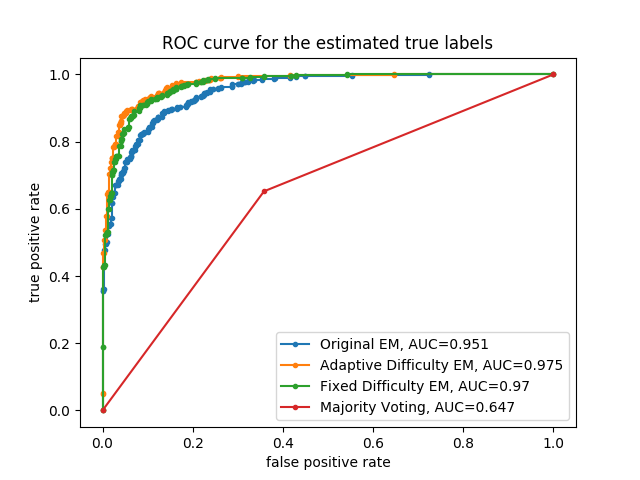
\includegraphics[width=5.0in]{image/roc_plot.png}
    \caption{ROC Curve for the estimated true labels. We compare our proposed methods with \textbf{Majority Voting} and \textbf{Original EM}} 
    \label{fig:gr}
\end{figure}

\textbf{2. Generalization of the learnt classifier}

From Table \ref{table:gt} we can see the generalization property of the learnt classifier is consistently well in all EM-based algorithms. Surprisingly, the proposed \textbf{Fixed Difficulty EM} algorithm increases the accuracy by a large margin but the AUC of it on the training set is inferior to \textbf{Adaptive Difficulty EM}. Our hypothesis is that the fixed imaged difficulty can play the role of regularization.

\begin{table}[H]
\caption{Guassian dataset: Accuracy of learnt classifier on test set}
\label{table:gt}
\begin{center}
\begin{tabular}{c c c c c }
		\toprule
		Method & Majority Voting & Original EM & Adaptive Difficulty EM & Fixed Difficulty EM	 \\
		\midrule
        Accuracy & $93.6 \pm 0.05$  & $94.00 \pm 0.11$ & $93.9 \pm 0.15$ & $\bm{94.4 \pm 0.13}$ \\
		\bottomrule
\end{tabular}
\end{center}
\end{table}

\textbf{3. Estimated expertise}

The actual sensitivity and specificity of each expert is marked as blue dots in Figure \ref{fig:ge}. We can see that the estimated expertise of our proposed EM algorithms is much closer to the actual values of sensitivity and specificity than the original EM algorithm. Moreover, we find that the estimated expertise of the two proposed algorithm is close. So different interpretations of image difficulty do not change the updating trajectory of experts' parameters much. We use $\alpha = \sigma (\frac{\bm{\lambda}^{1}}{4})$ and $\beta = \sigma(\frac{\bm{\lambda}^{2}}{4})$to recover the sensitivity and specificity of experts.

\begin{figure}[H]
    \centering
    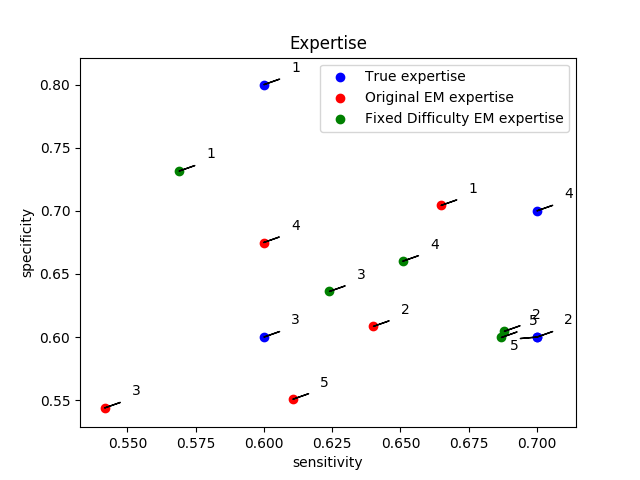
\includegraphics[width=5in]{image/expertise_g.png}
    \caption{Estimated Expertise on Gaussian dataset. The numbers denote corresponding experts. The expertise of \textbf{Adaptive Difficulty EM} and \textbf{Fixed Difficulty EM} is very close, so we only plot one of them. } 
    \label{fig:ge}
\end{figure}


\subsection{Dogs vs. Cats dataset}

In this experiments, the expert label real-world 2-class dataset. The experiment set up is almost the same as the two-dimension Gaussian mixture dataset except that the classifier used in this experiment is a four-layer convolutional neural network, and we use a pre-trained four-layer convolutional neural network to synthesis image difficulty, i.e the more uncertain the pretrained classifier is the more difficult this data point is.
We manually split the dataset into a $12,500$-image training set and a $12,500$-image test set to both test the accuracy of the estimated ground truth on the training set and the generalization performance of the learnt classifier on the test set.

\subsubsection{Structural Label}
Table \ref{table:dt}, Figure \ref{fig:dr} and Figure \ref{fig:de} summarize the results. The proposed \textbf{Fixed Difficulty EM} algorithm performs well both on estimating true labels and the generalization. The estimated expertise of \textbf{Original EM} marginally closer to the ground-truth expertise. 

We can see that \textbf{Majority Voting} can not converge in this case, and \textbf{Original EM} converges poorly. Actually, \textbf{Original EM} even can not converge in some experiments.


\begin{table}[htp]
\caption{Dogs vs. Cats dataset: Accuracy of learnt classifier on test set}
\label{table:dt}
\begin{center}
\begin{tabular}{c c c c c }
		\toprule
		Method & Majority Voting & Original EM & Adaptive Difficulty EM & Fixed Difficulty EM	 \\
		\midrule
        Accuracy & $50.0 \pm 0.0$  & $60.2 \pm 9.1$ & $70.4 \pm 0.9$ & $\bm{74.3 \pm 1.7}$ \\
		\bottomrule
\end{tabular}
\end{center}
\end{table}

\begin{figure}[htb]
    \centering
    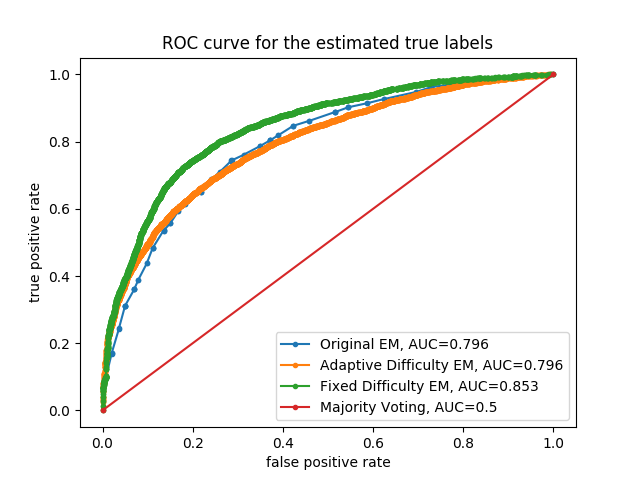
\includegraphics[width=5.5in]{image/roc_plot_dog.png}
    \caption{ROC Curve for the estimated true labels. We compare our proposed methods with \textbf{Majority Voting} and \textbf{Original EM}} 
    \label{fig:dr}
\end{figure}

\begin{figure}[htb]
    \centering
    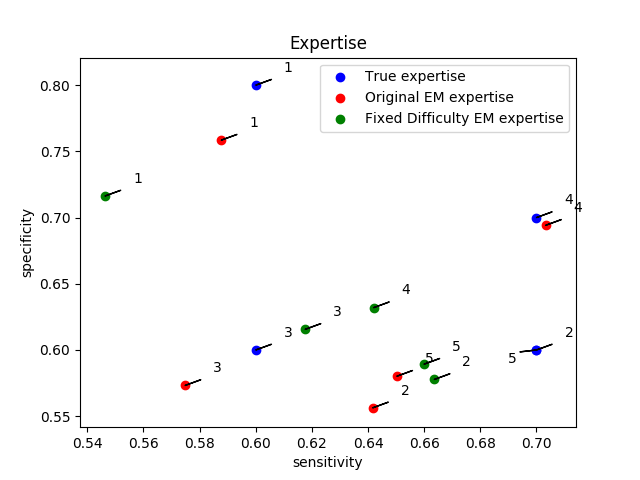
\includegraphics[width=5.5in]{image/expertise_dog.png}
    \caption{Estimated Expertise on Dogs vs Cats dataset. The numbers denote corresponding experts. The expertise of \textbf{Adaptive Difficulty EM} and \textbf{Fixed Difficulty EM} is very close, so we only plot one of them. } 
    \label{fig:de}
\end{figure}

\subsubsection{Non-structural Label}
Since in the experiments above, we use our assumption to synthesize the experts' labels, which is very structural. So we would like to compare these methods under settings that may be closer to real world, where the labels tend to be less structural. In such settings, with regard to every datapoint, an expert makes mistakes with probability $\frac{1}{3+k}$, where k is uniformly sampled from $\{0,1,2,3,4,5\}$. It should be noted that, to a single expert, the error probabilities corresponding to different images are also different. We only compare the generalization ability of the learnt classifier. The result is shown in Table \ref{table:rt}. The proposed algorithms still dominate other algorithms in this setting. The other two algorithms can not converge using non-structural labels.

\begin{table}[htp]
\caption{Non-structural label: Accuracy of learnt classifier on test set}
\label{table:rt}
\begin{center}
\begin{tabular}{c c c c c }
		\toprule
		Method & Majority Voting & Original EM & Adaptive Difficulty EM & Fixed Difficulty EM	 \\
		\midrule
        Accuracy & $50.0 \pm 0.0$  & $50.6 \pm 0.6$ & $76.7 \pm 0.8$ & $\bm{78.2 \pm 0.3}$ \\
		\bottomrule
\end{tabular}
\end{center}
\end{table}

\section{Conclusion and Outlook}
As an amelioration of \cite{raykar2010learning}, we present two EM algorithms for data that has different difficulty, which is a more natural setting in reality. To empirically verify the advantage of our algorithm, we conduct ablation study on synthesized data and real world data. Our methods outperform original method under both situation.

There is still room for improvement. The initialization of EM algorithm is a long-standing problem as EM algorithm only converges to one of its local minima. Some previous work \cite{zhang2014spectral} made discussions about this issue, which can be one of our next research target. What's more,  \cite{liu2012variational} tackles crowdsourcing problem with graphical models from a variational inference view, which is quite distinctive and worth further exploration.

{\small
\section*{Contribution}
Tianyuan Zhang has tried to use web crawler technique to collect data, but unfortunately failed out of the low qualification of images from the internet. Yilun Xu chose the topic and baseline, and at the meantime he conduct the experiment of Dogs & Cats which is the most complicated ones. The two algorithms are put forward by Weiyi Zhang and Tianyuan Zhang. Experiments are designed by Yilun Xu and Tianyuan Zhang.  Dinghuai Zhang wrote the article with Weiyi Zhang, besides he conduct the simple experiment of Guassian toy model. The computational resource is supplied by Tianyuan Zhang. The github repo is maintained by Yilun Xu right now.
}

\bibliography{ref} 
\appendix
\section{Experiment Details}
\subsection{The generation of datapoint difficulty and expert parameters}

\paragraph{Two-dimensional Gaussian Mixture dataset} Denote ground-truth Bayesian classification boundary as $\bm{w}$ and datapoint $i$ as $x_i$, and the synthesized datapoint difficulty $\mu_i = \frac{1}{1+w^Tx_i}$.

\paragraph{Dogs vs Cats dataset} We pre-trained a neural network $f$ and use the ouput of $\mu_i = f(x_i)$ w.r.t datapoint i as the image difficulty.

The expert parameters is calcualted by $\bm{\lambda^1} = 4\log{\frac{\alpha}{1-\alpha}}$ and $\bm{\lambda^2} = 4\log{\frac{\beta}{1-\beta}}$, which is the inverse of $\alpha = \sigma\lbrace\bm{\lambda}^{1}(p-1/2)^{2}\rbrace$ and $\beta = \sigma\lbrace\bm{\lambda}^{2}(p-1/2)^{2}\rbrace$ where $p=1$ or $p = 0$.

\subsection{Network Architecture}

The  architecture of the four-layer neural network is:

conv1-relu-maxpooling + conv2-relu-maxpooling + conv3-relu-maxpooling + conv4-relu-maxpooling + batch normalization + fc-relu-dropout + fc + softmax

\subsection{Initialization} 

For all EM based algorithm, we initialize the parameters $\{\alpha,\beta\}$ using the method in \cite{raykar2010learning}, then initialize $\{\bm{\lambda}\}$.

\begin{align}\label{initial}
	\alpha^r = \log{\frac{\sum\limits_{i=1}^N Q(y_i=c)\mathbbm{1}(y_i^r=1)}{\sum\limits_{i=1}^N Q(y_i=1)}}\\
	\beta^r = \log{\frac{\sum\limits_{i=1}^N Q(y_i=0)\mathbbm{1}(y_i^r=0)}{\sum\limits_{i=1}^N Q(y_i=0)}}\\
	\bm{\lambda_r}^1 = 4* \log{\frac{\alpha^r}{1-\alpha^r}} \\
	\bm{\lambda_r}^2 = 4* \log{\frac{\beta^r}{1-\beta^r}}
\end{align}

where $\mathbbm{1}(y_i^m=c')=1$ when $y_i^m=c'$ and $\mathbbm{1}(y_i^m=c')=0$ when $y_i^m\neq c'$ and N is the total number of datapoints. We average all crowdsourced labels to obtain $Q(y_i=c) := \frac{1}{R}\sum\limits_{r=1}^R \mathbbm{1}(y_i^r=c)$.



\end{document}

